\documentclass[12pt]{article}
\author{Alex Ho}
\title{FYS4150 - Computational Physics \\ Project 1}
\usepackage{listings}
\usepackage{graphicx}
\usepackage{verbatim}
\usepackage{amsmath}
\usepackage[utf8]{inputenc}
\usepackage[english, norsk]{babel}
\usepackage{xcolor}
\usepackage{hyperref}

\lstset{
language=Python,
basicstyle=\ttfamily,
otherkeywords={self},             
keywordstyle=\ttfamily\color{blue!90!black},
keywords=[2]{True,False},
%keywords=[3]{ttk},
keywordstyle={[2]\ttfamily\color{blue!90!black}},
emph={MyClass,__init__},          
emphstyle=\ttfamily\color{red!80!black},    
stringstyle=\color{blue!90!black},
showstringspaces=false,
commentstyle=\color{blue!90!black},
breaklines=true,
tabsize=3,
moredelim=**[is][\color{blue}]{@}{@}
}

\begin{document}
\maketitle
\section{Introduction}
Many of the important differential equations in science are second order differential equation. One example that we will use is Poisson's equation from electromagnetism. It tells us how electrostatic potential arises by a given charge distribution. In this project we will look at a general one-dimensional Poisson equation given as
\begin{align}
-u''(x) = f(x)
\end{align}
We want to develop different algorithms that solves this equation, and then compare them to see which one of them is the most efficient in terms of computing speed. By doing so, we will have to analyse the number of floating point operations that these algorithms have to do in order do compute our desired result.

%We want to develop different algorithms that solves this equation, and we also want to see which algorithm is the most efficient, in terms of computing time, by analysing the number of floating point operations each algorithm does. 

%We will in this project solve the one-dimensional Poisson equation, given as
%\begin{align}
%-u''(x) = f(x)
%\end{align}
%numerically, with Dirichlet boundary conditions by rewriting the Poisson equation to a set of linear equations. In this project, we will also focus on memory allocation, floating point operations in our numerical algorithm and compare the algorithms that we use in the project.  The method section is divided in multiple parts, where each part has a different task to be solved.
\section{Method}
\subsection*{a) Rewriting to a set of linear equations}
We can discretize the Poisson equation as
\begin{align}
-v''(x) &= f(x)\\ \nonumber
\implies -\frac{v_{i+1} + v_{i-1} - 2v_i}{h^2} &= f_i
\end{align}
Where $f_i = f(x_i)$, $v_{i+1}=v(x_{i+1}),$ etc. for $i=1,2,...,n$. Multiply $h^2$ on both sides, we get the following
\begin{align}
2v_i - v_{i+1} - v_{i-1} = \tilde{f_i}, \quad \tilde{f_i} = h^2f_i
\end{align}
Since this is for $i = 1,2,..,n$, one can write this as a set of linear equations
\begin{align}
2v_1 - v_2 = \tilde{f_1} \nonumber \\ 
2v_2 - v_3 - v_1 = \tilde{f}_2 \nonumber \\
2v_3 - v_4 - v_2 = \tilde{f}_3 \nonumber \\
\vdots \nonumber \\
2v_n - v_{n-1} = \tilde{f}_n
\end{align}
We know from the boundary conditions that $v_0 = v_{n+1} = 0$, so we do not include them in the algorithm. We can clearly see a pattern here. This set of linear equation can be written in the form
\begin{align}
\mathbf{A}\mathbf{v} = \mathbf{\tilde{f}}
\end{align}
Where
\begin{align}
\mathbf{v} = 
\begin{pmatrix}
v_1 \\
v_2 \\
\vdots \\
v_n
\end{pmatrix}
\qquad
\mathbf{\tilde{f}} =
\begin{pmatrix}
\tilde{f}_1\\
\tilde{f}_2\\
\vdots \\
\tilde{f}_n
\end{pmatrix}
\end{align}
And the tridiagonal $n \times n$ matrix as
\begin{align}
\mathbf{A} =
\begin{pmatrix}
2 & -1 & 0 & \cdots & \cdots & 0 \\
-1 & 2 & -1 & 0 & \cdots & \cdots \\
0 & -1 & 2 & -1 & 0 & \cdots \\
\cdots & \cdots & \cdots & \cdots & \cdots & \cdots \\
0 & \cdots & \cdots & -1 & 2 & -1 \\
0 & \cdots & \cdots & 0 & -1 & 2
\end{pmatrix}
\end{align}
We are also given the source term as $f(x) = 100e^{-10x}$ and that the closed-form solution, given the same interval and boundary conditions, is $u(x) = 1 - \left(1-e^{-10} \right)x - e^{-10x}$. This can easily be shown:
\begin{align}
-u''(x) &= -\frac{d^2}{dx^2} \left( 1 - \left(1-e^{-10} \right) x - e^{-10x} \right) \nonumber \\
&= - \frac{d}{dx}\left((1-e^{-10}) + 10e^{-10x} \right) \nonumber\\
&= -\left(-100e^{-10x} \right) = f(x)
\end{align}
\subsection*{b) Forward and backward substitution}
Our matrix $\mathbf{A}$ can be written in terms of one-dimensional vectors $a,b$ and $c$ with the length $i=1:n$. The linear equation is then
\begin{align}
\begin{pmatrix}
b_1 & c_1 & 0 & \cdots & \cdots & \cdots \\
a_1 & b_2 & c_2 & 0 & \cdots & \cdots \\
0 & a_2 & b_3 & c_3 & 0 & \cdots \\
 & 0 & \cdots & \cdots & \cdots & \cdots \\
 & & & a_{n-2} & b_{n-1} & c_{n-1} \\
 & & & & a_{n-1} & b_n
\end{pmatrix}
\begin{pmatrix}
v_1 \\
v_2 \\
v_3 \\
\vdots \\
v_{n-1} \\
v_n
\end{pmatrix}
=
\begin{pmatrix}
\tilde{f}_1 \\
\tilde{f}_2 \\
\tilde{f}_3 \\
\vdots \\
\tilde{f}_{n-1} \\
\tilde{f}_n
\end{pmatrix}
\end{align}
We want to write an algorithm to solve the values of $v_i$, assuming different values for the matrix elements $a_i, b_i, c_i$. We also want to find the number of floating point operations (flops) that is needed to solve the given algorithm.

Let us start by writing out the linear equation to be in the form similar to (5)
\begin{align}
b_1v_1 + c_1v_2 &= \tilde{f}_1 \\
a_1v_1 + b_2v_2 + c_2v_3 &= \tilde{f}_2 \\
a_2v_2 + b_3v_3 + c_3v_4 &= \tilde{f}_3 \\
\vdots \nonumber \\
a_{n-2}v_{n-2} + b_{n-1}v_{n-1} + c_{n-1} v_n &= \tilde{f}_{n-1}\\
a_{n-1}v_{n-1} + b_n v_n &= \tilde{f}_n
\end{align}
Starting with (10) and (11), we first multiply (10) with $a_1/b_1$ and then subtract (11) with the new (10) (after the multiplication), we get
\begin{align}
a_1v_1 + \frac{c_1 a_1}{b_1}v_2 &= \tilde{f}_1\frac{a_1}{b_1}  \\
a_1v_1 + b_2v_2 + c_2v_3 - (a_1v_1 + \frac{c_1 a_1}{b_1} v_2) &= \tilde{f}_2 - \tilde{f}_1\frac{a_1}{b_1}
\end{align}
Multiply $b_1/a_1$ on (15), and with a little rewriting we arrive to
\begin{align}
b_1v_1 + c_1v_2 &= \tilde{f}_1 \\
\tilde{b_2}v_2 + c_2v_3 &= F_2
\end{align}
Where I have now defined $\tilde{b}_2 = b_2 - \frac{c_1 a_1}{b_1}$ and $F_2 = \tilde{f}_2 - \tilde{f}_1\frac{a_1}{b_1}$. Let us now continue by looking at (12) and (19), that is
\begin{align}
\tilde{b}_2 v_2 + c_2 v_3 &= F_2 \\
a_2 v_2 + b_3 v_3 + c_3 v_4 &= \tilde{f}_3
\end{align}
Doing the same trick as we did previously, we multiply $a_2/\tilde{b}_2$ on equation (19) and then subtract that on (20). Rewriting a little bit we end up with
\begin{align}
\tilde{b}_2 v_2 + c_2 v_3 &= F_2 \\
\tilde{b}_2 v_3 + c_3v_4 &= F_3
\end{align}
Here I have defined $\tilde{b_3} = b_3 - \frac{c_2 a_2}{\tilde{b_2}}$ and $F_3 = \tilde{f_3} - F_2\frac{a_2}{\tilde{b_2}}$. One can continue to do this, but we can clearly see a pattern here, which results to these general expressions
\begin{align}
\tilde{b}_i &= b_i - \frac{c_{i-1} a_{i-1}}{\tilde{b}_{i-1}}\\
F_i &= \tilde{f}_i - F_{i-1}\frac{a_{i-1}}{\tilde{b}_{i-1}}, \qquad \text{for } i=2,...n
\end{align}
This is known as \textit{Forward Substitution}. For $i=1$, we need to explicitly define that $\tilde{bn_1} = b_1$ and $F_1 = \tilde{f_1}$. This is mostly because values like $c_0$ and $a_0$ are outside our interval.\footnote{Not to be confused with the index notation in C++ and Python, where intervals goes as $x_0, x_1, ... , x_{n-1}$}. The number of floating point operations (flops) for these two steps combined is	 $6$ flops. Both steps do one subtraction, one multiplication and one division, which means that each of them do $3$ flops, and the total will therefore be $6$ flops.

The next step is to find an algorithm to find the values of $v_i$. From the calculations above, our linear equations are as following
\begin{align}
b_1v_1 + c_1v_2 &= \tilde{f}_1 \\
\tilde{b}_2v_2 + c_2v_3 &= F_2 \\
\tilde{b}_3v_3 + c_3v_4 &= F_3 \\
\vdots \nonumber \\
\tilde{b}_{n-1} v_{n-1} + c_{n-1}v_n &= F_{n-1} \\
\tilde{b}_nv_n &= F_n
\end{align}
From (29) we have that $v_n = F_n/\tilde{b}_2$, which is the $"$initial" value of $v$ and we will have to calculate backwards to get all the values of $v_i$. Equation (28) gives us the relation:
\begin{align*}
v_{n-1} = \frac{1}{\tilde{b}_{n-1}}\left(F_{n-1}-c_{n-1}v_n \right)
\end{align*}
In terms of $i$'s, this will become
\begin{align}
v_{i-1} = \frac{1}{\tilde{b}_{i-1}}\left(F_{i-1} - c_{i-1}v_i \right), \quad \text{for } i = n,n-1,...,2
\end{align}
This is known as \textit{Backward Substitution}. The number of flops in this case will be $3$ flops.Like Forward substitution, we have one subtraction, one multiplication and one division. The number of flops for both Forward substitution and Backward substitution is $9$ flops. We also have to keep in mind that we do these calculations $n$ times, so the total number of flops for all $n$ equations is $9n$ flops.
\subsection*{c) Specialized algorithm}
We now use the fact that our matrix $\mathbf{A}$ has identical matrix elements along the diagonal and the non-diagonal elements are also identical (but different from the diagonal one). With our specific tri-diagonal matrix $\mathbf{A}$, we will specialize our algorithm from the previous task to solve our linear equation.

Let us first look at the forward substitution algorithm for $\tilde{b}_i$, we had
\begin{align}
\tilde{b}_i = b_i - \frac{c_{i-1}a_{i-1}}{\tilde{b}_{i-1}}
\end{align}
With the non diagonal elements as $a_i = c_i = -1$ and $b_i = 2$. With the initial value $\tilde{b}_1 = b_1 = 2$, we can write out every $\tilde{b}_i$ value, but after a few steps, one can see a pattern and we end up with
\begin{align}
\tilde{b}_2 &= 2 - \frac{1}{2} = \frac{3}{2} \nonumber \\
\tilde{b}_3 &= 2 - \frac{1}{\frac{3}{2}} = \frac{4}{3} \nonumber \\
\tilde{b}_4 &= 2 - \frac{1}{\frac{4}{3}} = \frac{6}{5} \nonumber \\
\vdots \nonumber \\
\tilde{b_i} &= \frac{i+1}{i}, \quad \text{for } i = 1,2,...,n
\end{align}
The next step in the forward substitution algorithm is then
\begin{align}
F_i &= \tilde{f}_i - F_{i-1}\frac{a_{i-1}}{\tilde{b}_{i-1}}  \nonumber \\
\implies F_i &= \tilde{f}_i + \frac{F_{i-1}}{\tilde{b}_{i-1}}, \quad \text{for } i=2,...,n
\end{align}
Where the initial value is $F_1 = \tilde{f}_1$. Finally, the backward substitution algorithm can be simplified to
\begin{align}
v_{i-1} &= \frac{1}{\tilde{b}_{i-1}}(F_{i-1}-c_{i-1}v_i) \nonumber \\
\implies v_{i-1} &= \frac{1}{\tilde{b}_{i-1}}(F_{i-1} + v_i), \quad \text{for } i = n, n-1, ..., 2
\end{align}
With the initial value $v_{n} = F_n/\tilde{b}_n$. The number of flops for all three steps is $2$ flops. Each of them do one addition and one division. However, since the values of $\tilde{b}_i$ is calculated beforehand, we do not have to take into account the calculations of these values, as they can be vectorized and quickly calculated in C++. Therefore, the number of flops is only calculated by the second part of the forward substitution and backward substitution. Because of this, and keeping in mind that we are solving these equations $n$ times, then the total number of flops is $4n$ flops. This is roughly half the flops required to solve our equation compared to the general method, so we can expect that this method computes faster.

\subsection*{d) Calculating relative error}
We are tasked to calculate the relative error given as
\begin{align*}
\epsilon_i = log_{10}\left(\frac{v_i - u_i}{u_i} \right)
\end{align*}
as a function of $log_{10}(h)$. Different values of $h$ corresponds to different values of $n$. We will in this project use the values of $n$ from $n=10$ up to $n=10^7$. One should keep in mind that the values of $u_i$ can be very small near the end points, which can give a very large relative error.

\subsection*{e) LU decomposition}
The LU decomposition is done by using the \textit{lib.cpp} file that is provided this course. The idea of LU decomposition is to factorize our matrix as a product of two matrices, where one is a lower triangular matrix and the other is an upper triangular matrix. That is
\begin{align}
\mathbf{A} = \mathbf{L}\mathbf{U}
\end{align}
Where
\begin{align*}
\mathbf{L} =
\begin{pmatrix}
1 & 0 & \cdots & \cdots & \cdots \\
l_{21} & 1 & 0 \cdots & \cdots \\
l_{31} & l_{32} & 1 & 0 & \cdots \\
\vdots & \cdots & & & \\
l_{n1} & \cdots & & l_{n,n-1} & 1 \\
\end{pmatrix}, \quad
\mathbf{U} =
\begin{pmatrix}
u_{11} & u_{12} & \cdots & \cdots & u_{1n} \\
0 & u_{22} &\cdots & & \vdots \\
0 & \cdots & & & \\
& & \ddots & & \\
\cdots& \cdots & & & u_{nn}
\end{pmatrix}
\end{align*}
We will then have to evaluate the values of $l_{ij}$ and $u_{ij}$. This step requires roughly $(2/3)n^3$ flops, which is quite a lot already. However, a couple more steps has to be done to get our desired results. We now have two sets of equations given as
\begin{align}
\mathbf{L}\mathbf{w} = \mathbf{y} \\
\mathbf{U}\mathbf{x} = \mathbf{w}
\end{align}
Both these equations requires roughly $\mathcal{O}(n^2)$ flops. So the total number of flops is roughly $\mathcal{O}(\frac{2}{3} n^3$) flops, which is significantly larger than what is required for our general algorithm. We can expect that it will take a lot more computing time once $n$ gets larger.

We are also asked if it is possible to run LU decomposition with $10^5 \times 10^5$ matrix elements. This is something that I will not try for this project as, according to the lecture notes, it takes roughly 16 minutes to run this method for $n=10^4$. Running this with $n=10^5$ will probably explode (figuratively) my computer.
\section{Implementation}
I have used both C++ and Python to solve this project. The strategy is to use C++ to develop and algorithm, do the calculations and save the results to a text file. Once I have the results, I use Python mostly to plot the values that was calculated in C++. I will also calculate the relative error in python and then save it to a text file. All files for this project can be found in the GitHub repository \url{https://github.com/AHo94/FYS3150_Projects/tree/master/Project1}.

For the general algorithm, I will assume that the values along the diagonal are the same. This is to compare the results between the general and special method.

Since we are only calculating the values of $i=1,...,n$, I have ignored the points at $i=0$ and $i=n+1$ in the C++ program. To compensate for that (and also to make sure we have the boundaries), I will have to add these points after the data calculations. This is done in the Python script, where I increase the array by $2$ and then set the boundary conditions.

One important note is that the indexes in C++ and Python runs through $i=0$ to $i=n-1$. So equations like equation (32) has to be modified with respect to this, so calculating   $\tilde{b}_i$ for the special case is in C++
\begin{align}
\tilde{b}_i = \frac{i+2}{i+1}, \quad \text{for } i=0,1,...,n-1
\end{align}

I have also made sure that I only plot at most 1000 points. For parts where I calculate with, for example $n=10^6$ points, the number of data points saved will create a very very large text file. Also, plotting that many points is not necessary when $1000$ points is sufficient.

\section{Results}
Figure (1) and (2) shows the results of the dataset in the general algorithm. As we can see, the algorithm starts to converge from below to the exact solution. As we increase the number of points, the algorithm yields practically the same data points as the exact solution.

\begin{figure}[hbtp]
\centering
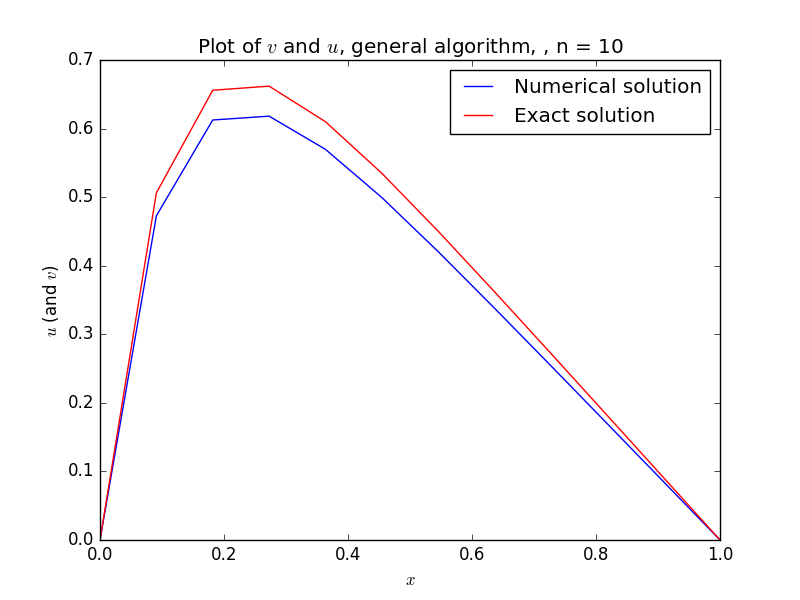
\includegraphics[scale=0.5]{Data_plots/General_data_n10.png}
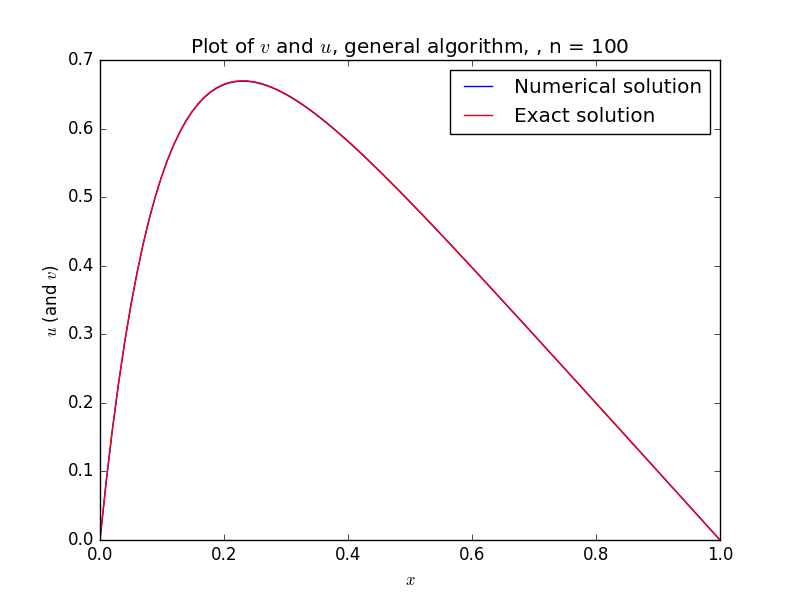
\includegraphics[scale=0.5]{Data_plots/General_data_n100.png}
\caption{Graphs showing the results of the general algorithm as a function of $x$, for $n =$ 10 and 100}
\end{figure}

\begin{figure}[hbtp]
\centering
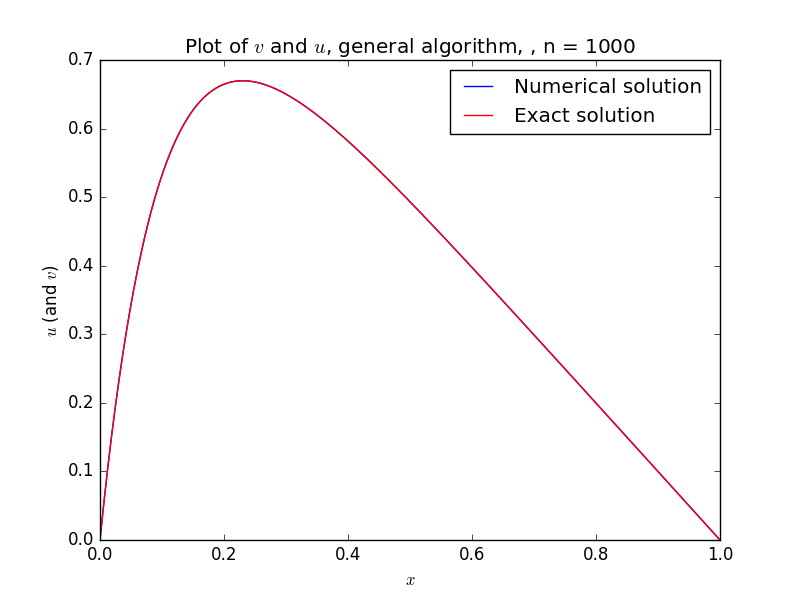
\includegraphics[scale=0.5]{Data_plots/General_data_n1000.png}
\caption{Graph showing the result of the general algorithm  as a function of $x$, with $n=$1000}
\end{figure}

Figure (3) and (4) shows the results from the specialized algorithm, where we know the diagonal elements beforehand. There is in fact nothing different here as both methods gave the same results (see table 2). Plots for $n=10^4, 10^5$ and $10^6$ can be found in the GitHub repository under  the Data\_plots folder.

\begin{figure}[hbtp]
\centering
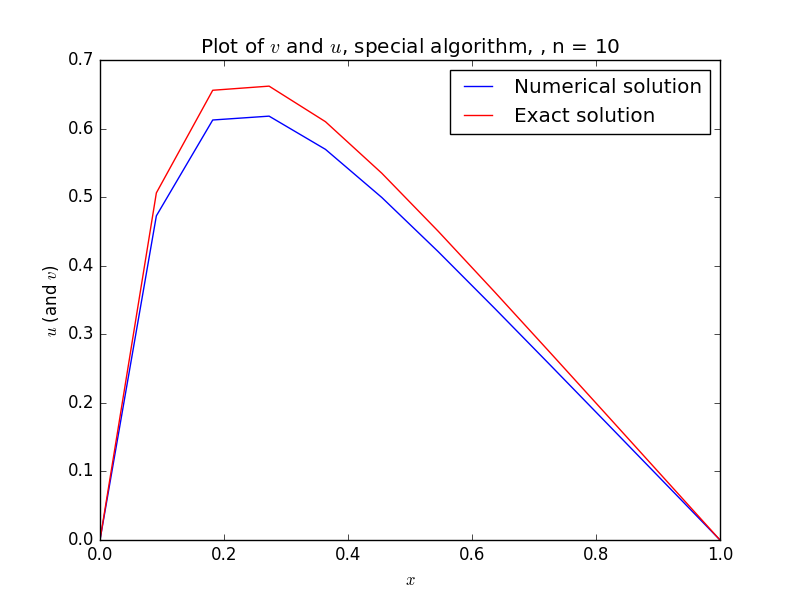
\includegraphics[scale=0.5]{Data_plots/Simplified_data_n10.png}
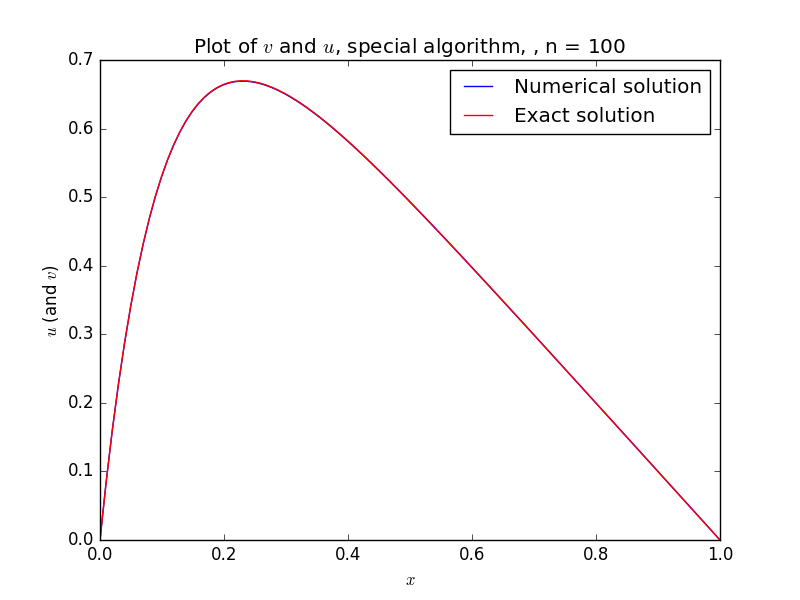
\includegraphics[scale=0.5]{Data_plots/Simplified_data_n100.png}
\caption{Graphs showing the results of the specialized algorithm as a function of $x$, for $n =$ 10 and 100}
\end{figure}

\begin{figure}[hbtp]
\centering
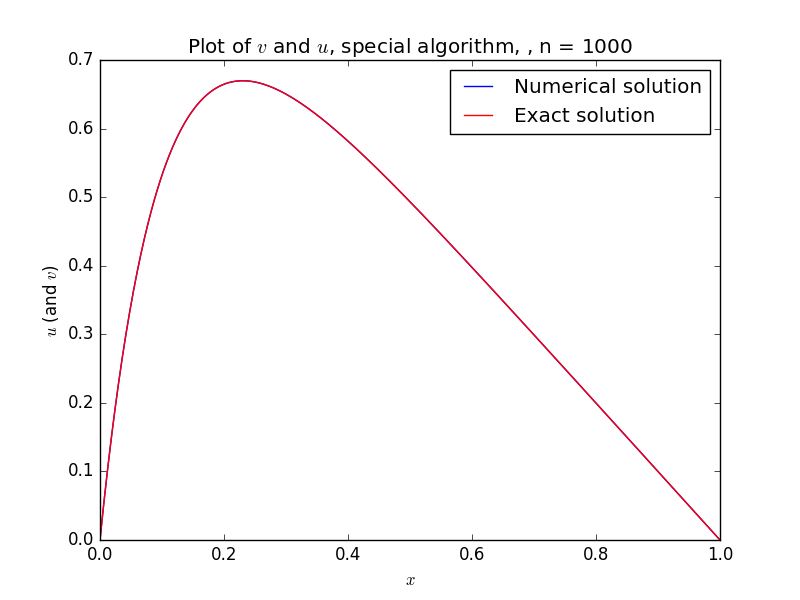
\includegraphics[scale=0.5]{Data_plots/Simplified_data_n1000.png}
\caption{Graph showing the result of the specialized algorithm as a function of $x$ with $n=$1000}
\end{figure}

Figure (5) Shows the relative error between $u_i$ and $v_i$ for different step lengths (equivalent to different values of $n$). Both axes are plotting in $log_{10}$ scale. The results seems a little weird to me, as I expect more of a $\vee$-like shape for the relative error. We can of course expect that the relative error is larger for a smaller value of $n$, but one would also expect a large error for larger values of $n$ as well. This is because the step lengths would be so small, we would have many small values for the $x$ values. This would then result to many small values for our exact solution $u(x)$ which could possibly affect the relative error $\epsilon_i$. Table (1) shows the values of the relative error.

\begin{table}
\begin{center}
	\begin{tabular}{| l | l |}
		$log_{10}(h)$ & $log_{10}(\epsilon_i)$ \\ \hline
		-1.17968824808 &  -1.04139268516 \\
		-3.08623007481 &  -2.00432137378 \\
		-4.93468086898 &  -3.00043407748 \\
		-3.99532916844 &  -4.00004342728 \\
		-4.85661864816 &  -5.00000434292 \\
		-5.26615428789 &  -6.00000043429 \\
		-5.36464463167 &  -7.00000004343 \\
		 \hline
	\end{tabular}
\caption{Data values of the relative error with the corresponding $h$ values, both in $log_{10}$ scale.}
\end{center}
\end{table}

\begin{figure}[hbtp]
\centering
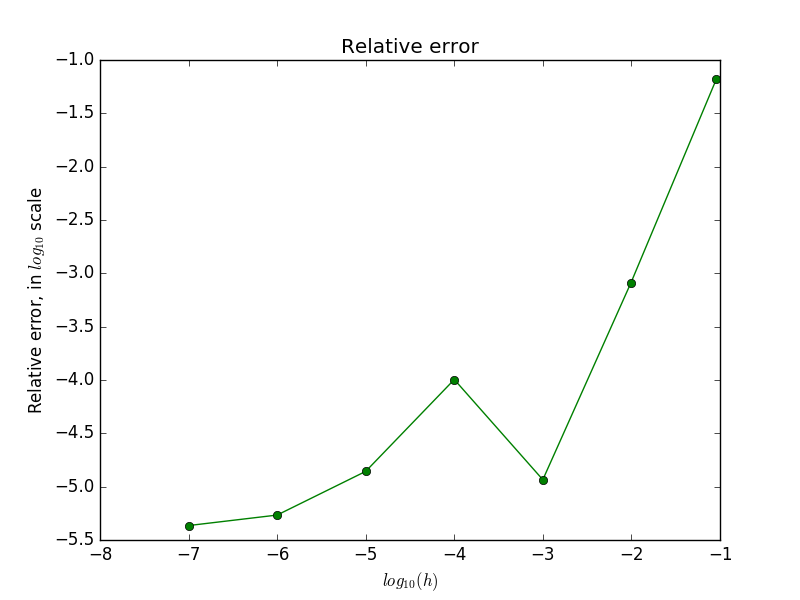
\includegraphics[scale=0.5]{Data_plots/Relative_error.png}
\caption{Plot of the relative error as a function of $log_{10}(h)$}
\end{figure}

The LU decomposition has not been plotted, as the dataset from this algorithm is exactly the same as the general and special algorithm that we developed. Table (2) shows the calculated data from these methods. The dataset can be found in the following GitHub link: \url{https://github.com/AHo94/FYS3150_Projects/tree/master/Project1/build-Project1_cpp-Desktop_Qt_5_7_0_MinGW_32bit-Debug} 

\begin{table}
\begin{center}
	\begin{tabular}{| l | l | l | l |}
		$x$ & $v_g$ & $v_s$ & $v_{LUD}$ \\ \hline
		0.0909091 & 0.472737 & 0.472737 & 0.472737 \\
		0.181818  & 0.612506 & 0.612506 & 0.612506 \\
		0.272727 &  0.618127 & 0.618127& 0.618127\\
		0.363636 &  0.5697 & 0.5697& 0.5697\\
		0.454545 &  0.499497 & 0.499497& 0.499497\\
		0.545455 &  0.420522 & 0.420522& 0.420522\\
		0.636364 &  0.338012 & 0.338012& 0.338012\\
		0.727273 &  0.254078 & 0.254078& 0.254078\\
		0.818182 &  0.169571 & 0.169571& 0.169571\\
		0.909091 &  0.0848319 & 0.0848319& 0.0848319 \\ \hline
	\end{tabular}
\caption{Comparison of calculated data between the general $v_g$ algorithm, special $v_s$ algorithm and LU decomposition $v_{LUD}$ for $n=10$ points.}
\end{center}
\end{table}

The CPU time of these three methods, printed out from the program, are shown in blue text below:
\begin{lstlisting}
@Time elapsed for general algorithm: 5.3e-005s
Time elapsed for specialized algorithm: 1e-005s
Time elapsed for LU-decomp: 14s@
\end{lstlisting}
For the special algorithm, I have only calculated the CPU time for the $n=10,100,1000$ calculations it has done and ignored calculations with $n=10^4, 10^5, 10^6$. It would obviously take a longer time to compute the data if we have more points, so comparing the same amount of calculations would set a better example.

As we can see, the general algorithm takes slightly more time to finish compared to the special algorithm, as we expected. The CPU time for the LU decomposition algorithm was roughly 14 seconds. Again, LU decomposition uses a lot more flops to compute our equation, it is no surprise to us that it also took a lot longer to finish compared to the two other methods.
% This is not surprising to us, as the special method do less flops. The LU decomposition, on the other hand, takes a lot longer time to finish its calculation in comparison to the two previously mentioned other methods.

\section{Conclusion}
From the results, we can clearly see that using LU decomposition is not an ideal way to solve our linear equations, given that we know that our matrix $\mathbf{A}$ is a tridiagonal matrix. The best method for our matrix $\mathbf{A}$ was the specialized method that we implemented. Though, this was not really surprising because we know the specialized method used less floating point operations compared to the two other methods. 

However, even though the algorithm for the special case was faster, the time difference between this and the general algorithm is negligible. So, even if the elements along the diagonal were not the same, the general algorithm would still work incredibly well if our matrix is tridiagonal.

But what happens if the matrix is no longer tridiagonal? The general algorithm will no longer work, and we would perhaps have to use LU decomposition to solve the linear equations.
\section{References}
M. Hjort-Jensen, 2015, \textit{Computational Physics}, accessible at course GitHub repository; \url{https://github.com/CompPhysics/ComputationalPhysics/tree/master/doc/Lectures} (as of 14.09.16), 551 pages.
\end{document}